\chapter{Branching and Extinction}

\section{A Process in Which Every Individual Branches}

Chapter 15 grew a cluster by attachment to a structure that already existed, and Chapter 16 filled a lattice site by site. A third way of forming structure lets every existing element produce its own successors, independently of the others. The simplest rule of this kind is the Galton--Watson process. A single individual forms generation zero. Each individual in generation $g$ has a random number of offspring, drawn from one fixed distribution and independently of every other individual, and those offspring make up generation $g+1$. The record of who descended from whom is a rooted tree, and the tree is the object of interest, because a branching structure in a habitat such as a drainage pattern, a root system or a corridor network can be described in the same terms: a rule for how many children each node has, and nothing else.

For the version used here the offspring number is Poisson distributed with mean $m$. Four things must be stated for the process to be reproduced: the offspring distribution and its mean, the rule for stopping a run, the generator, and the seed. The stopping rule matters more than it first appears. A process with $m>1$ may grow without bound, and a process with $m\le 1$ dies out with certainty, but in a finite computation a run can only be stopped, and a run that has been stopped is not a run that has died out. The runs below stop at extinction, at $60$ generations, or when the tree reaches $20{,}000$ individuals, and each run is classified by which of the three happened. A run that reaches the size cap is counted as a survivor in the estimates below, which is an approximation: a tree of $20{,}000$ individuals could in principle still die out, and the probability of that is small and was not measured.

The code is in \texttt{branching.py}. The generator is NumPy's \texttt{default\_rng} seeded by an integer. A run from seed $4$ at $m=1.5$ was identical on repetition, and seed $5$ gave a different tree.

\section{The Extinction Law}

The classical result is that the extinction probability $q$ is the smallest non-negative solution of $q=f(q)$, where $f$ is the generating function of the offspring distribution. For Poisson offspring $f(q)=e^{m(q-1)}$, and the solution is $q=1$ for $m\le1$ and a value below one for $m>1$. The solution was computed by iterating $q\leftarrow e^{m(q-1)}$ from $q=0$, which converges to the smallest root, and then compared it with the fraction of runs that went extinct in an ensemble of $2000$ seeds at each $m$.

\begin{center}
\begin{tabular}{rrrrrr}
\toprule
$m$ & $q$ from the equation & Extinct fraction & Extinct & Size cap & Alive at 60\\
\midrule
0.8 & 1 & $1.0000\pm0.0000$ & 2000 & 0 & 0\\
1.0 & 1 & $0.9605\pm0.0044$ & 1921 & 0 & 79\\
1.2 & 0.6863 & $0.6775\pm0.0105$ & 1355 & 635 & 10\\
1.5 & 0.4172 & $0.4135\pm0.0110$ & 827 & 1173 & 0\\
2.0 & 0.2032 & $0.2090\pm0.0091$ & 418 & 1582 & 0\\
\bottomrule
\end{tabular}
\end{center}

The figures after $\pm$ are binomial standard errors. For $m=1.2$, $1.5$ and $2.0$ the measured fraction differs from the root of the equation by $0.8$, $0.3$ and $0.6$ standard errors, so the ensemble agrees with the equation to the precision of $2000$ runs, with the size-cap approximation included. The row for $m=1.0$ needs a separate reading. The fixed-point iteration for $m=1$ converges so slowly that its output after $2000$ steps, $0.999$, was not used, and the value $1$ in the table is the theoretical one. The measured extinct fraction, $0.9605$, falls below one only because $79$ runs were still alive when stopped at $60$ generations. Those are not survivors in the sense of the theorem. A process at the critical value dies out with certainty, but the time it takes is heavy tailed, and a cut at $60$ generations leaves a few percent still running. For critical processes with finite variance the probability of surviving to generation $n$ is known to fall roughly as $2/(\sigma^2 n)$, which is $0.033$ at $n=60$ for $\sigma^2=1$, against $0.0395$ measured. That formula is recalled from reading and was not derived, and the agreement is of the right size and no more precise than that.

Two lessons for any process run on a computer follow from the table. The classification of a run into extinct, capped and alive must be reported, because the three outcomes are different statements. And a result at the critical value of a parameter depends on the stopping rule, so a figure such as $0.9605$ is a property of the run length as much as of the process.

\section{Total Size at the Critical Value}

At $m=1$ every run is finite, so it has a total number of individuals $T$, and the distribution of $T$ has a heavy tail. For $4000$ seeds, with runs allowed up to $400$ generations and $100{,}000$ individuals, the fraction with $T\ge t$ was $0.6375$, $0.2677$, $0.0875$ and $0.0312$ for $t=2$, $10$, $100$ and $1000$. The product of this fraction with $\sqrt t$ was $0.902$, $0.847$, $0.875$ and $0.988$. A tail of the form $P(T\ge t)\propto t^{-1/2}$ would make the product constant, and the measured values are close to constant, within the sampling error of the last, which is about $0.09$ from $4000$ runs. A tail exponent of one half over three decades in $t$ is therefore consistent with the data. The longest critical tree among the first $300$ seeds that went extinct had $11{,}590$ individuals and the typical one far fewer, so the mean size is not a useful summary of a critical process. The exponent is a statement about this ensemble, and the constant in the tail, which was not compared with a theoretical value, is not claimed.

\section{One Realisation in Blender}

A realisation is a tree, and a tree is placed in Blender as one object per edge, all sharing one box mesh scaled to the length of the edge and rotated to its direction, in the manner of Chapters 5, 15 and 16. Each edge carries its generation as a custom property, one material reads it with an Attribute node, and the layout is the standard tidy one in which leaves have consecutive horizontal positions in depth-first order and each parent sits at the mean position of its children. The script is \texttt{branching\_blender.py}.

A critical realisation was chosen as the first seed whose run went extinct with between $150$ and $300$ individuals. The first such seed was $1$, with $166$ individuals, and the scene held $165$ edge objects, one mesh with $165$ users and one material. The edge objects formed a tree in the exact sense that there were $n-1$ edges, every node except the root appeared as a child exactly once, and every parent was created before its child, so there were no cycles. The generation stored on each edge equalled the generation recomputed from the edge list, the position of each edge matched the midpoint of its endpoints in the layout to $4\times10^{-6}$, and the tree regenerated from the stored seed and mean reproduced the scene individual for individual. The population by generation of this tree was $1,2,2,1,2,2,1,1,3,3,4,4,5,6,11,13,8,10,15,13,15,11,6,5,6,6,8,2$, so it reached generation $27$ and then ended, having never exceeded fifteen individuals in a generation. This is typical of the critical process, which survives for a long time at small width and then dies.

\begin{figure}[ht]
\centering
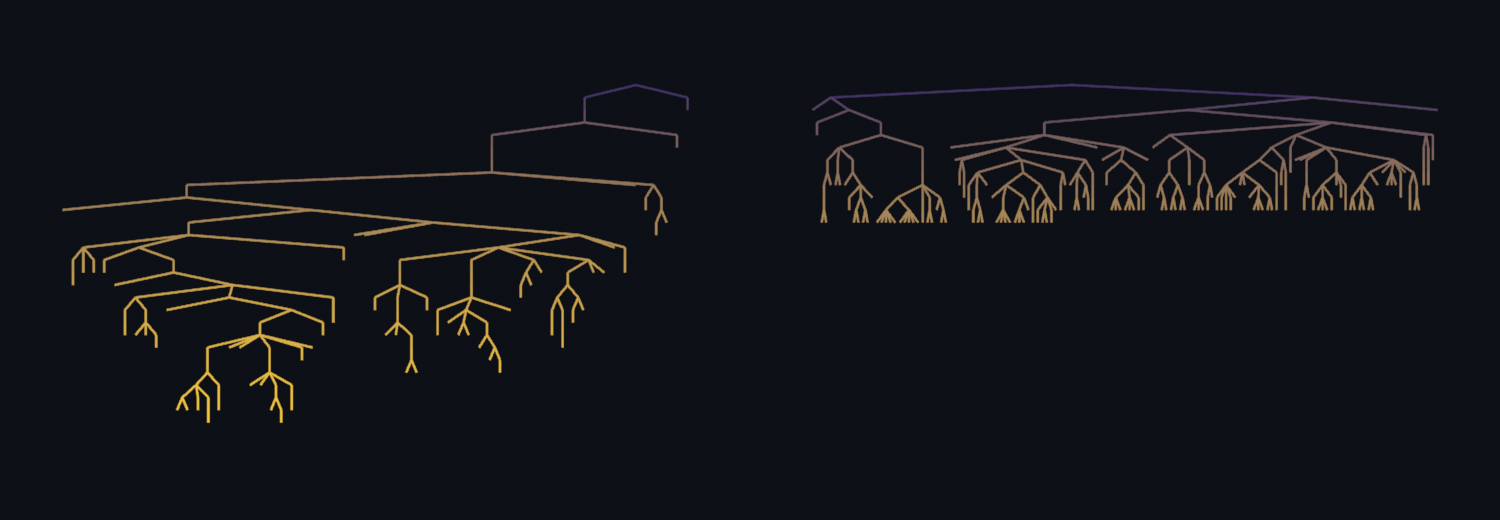
\includegraphics[width=\textwidth]{figs/fig17_trees.png}
\caption{Left, a critical realisation ($m=1$, seed $1$) that went extinct at generation $27$ with $166$ individuals. Right, a supercritical realisation ($m=1.5$, seed $1$) stopped at $300$ individuals, which reached generation $11$. Edges are coloured by generation from early (purple) to late (yellow), with one material and a colour scale running to generation $28$ in both trees. Each tree is drawn to the same width, so the horizontal scales differ.}
\end{figure}

The supercritical tree on the right was stopped at the size cap during a generation, so its last generation is incomplete, and the truncation falls on the later individuals by construction. It is shown to give the visual contrast of a wide and shallow tree against a narrow and deep one, and it is not a sample from which any statistic in this chapter was computed.

\section{What These Experiments Do Not Show}

All results are for Poisson offspring with five values of the mean, $2000$ runs at each in the extinction table and $4000$ at the critical value, with stopping rules stated above. Nothing was varied in the offspring distribution, so the agreement with the extinction equation does not show that the equation is the right description of a process with a different distribution, and the critical tail was not compared across distributions. The count of capped runs as survivors is an approximation whose error was not bounded. The $60$-generation cut produced the entire gap between the measured and the theoretical extinct fraction at $m=1$, and that attribution rests on the count of $79$ runs alive at the cut and was not tested by lengthening the run. The tail exponent was estimated by constancy of a product over four values of $t$ and not by a fit. The theoretical formulas for the critical process are recalled from reading. Finally, nothing here shows that any physical branching structure follows a branching process: independence of offspring, the absence of competition for space, and the lack of any geometry in the layout are assumptions of the rule, and the layout in the figure is a drawing of a tree, not a model of how the tree would occupy space.

\begin{exercise}[17.1: Another offspring law]
Replace the Poisson distribution by a distribution that takes the values $0$ and $2$ with equal probability, which has mean $1$ and a different variance. Measure the fraction alive at generation $60$ and compare it with the Poisson value. State what quantity the difference should be proportional to, and test the claim.
\end{exercise}

\begin{exercise}[17.2: Bound the size cap]
For $m=1.2$, rerun the extinction ensemble with caps of $2000$, $20{,}000$ and $200{,}000$ individuals, and report whether the extinct fraction changes by more than its standard error. State what that says about the survivor approximation.
\end{exercise}

\begin{exercise}[17.3: A branching rule with space]
Give each child a position displaced from its parent by a unit step in a random direction, and count the pairs of nodes closer than $0.3$ in trees of about $300$ individuals at $m=1.5$. State what the count says about whether the independence assumption could describe a structure that occupies the plane.
\end{exercise}

\begin{exercise}[17.4: Rebuild from the edge list]
Given only the edge objects in a saved scene, recover the number of individuals in each generation and test your recovery against the list printed in Section 17.4. Then delete one edge object and describe which checks of that section detect the loss.
\end{exercise}
